\documentclass[12pt, titlepage]{article}
\usepackage{preamble}
\addbibresource{referencias.bib}

\author{Francisco Pessoa, 1°EM A}
\affil{Colégio Ítaca}
\date{São Paulo, 27 de fevereiro de 2024}
\title{Experimentos sobre o crescimento de bolores}

\begin{document}
\maketitle

\section*{Resumo}
Esse experimento buscou analisar o surgimento e o crescimento de colônias de fungos em um caldo de água com amido de milho fervido, dividido em quatro placas de Petri, para que fossem analisadas diferentes possibilidades de surgimento e crescimento dos fungos. Uma das placas foi tampada imediatamente, outra foi resfriada e então tampada, uma foi deixada aberta em um saco plástico fechado com furos e outra foi deixada aberta e exposta ao ambiente. Notou-se que, quanto maior o contato com o ambiente externo, maior foi o desenvolvimento de microorganismos nas placas.

\section{Introdução teórica e objetivo}
\subsection{Biogênese, geração espontânea e abiogênese\label{intro-surg-vida}}
Durante a história da biologia, duas principais explicações para o surgimento da vida foram formuladas: a geração espontânea, hipótese que, previsivelmente, defende a geração de organismos vivos a partir de matéria não-viva, e a biogênese, teoria atualmente mais aceita que prevê que toda a vida é proveniente de algum ser vivo pré-existente. Com o avanço da metodologia científica e da tecnologia, hoje em dia a geração espontânea foi completamente desacreditada e obsoletada. Contudo, sua discussão é ainda pertinente visto que fez parte do pensamento biológico durante quase dois séculos e auxiliou substancialmente a constituição do pensamento e método experimental científico, além de ter influenciado na constituição religiosa de muitas sociedades passadas, como a Grécia antiga, sociedades islâmicas antigas e predominou no pensamento científico da Idade Média.

A hipótese da geração espontânea foi definitivamente descartada com o experimento do bico de cisne de Pasteur \cite{bsfi2019pasteur,enwiki:1195385720}, experimento que usou um recipiente cheio de caldo nutritivo mas que cuja única saída externa era um fino bico que se recurvava para baixo e depois para cima (o chamado \textit{bico-de-cisne}, veja figura \ref{bico-de-cisne}). Deste modo, haveria circulação de ar dentro do frasco, mas ainda sim não surgiram microorganismos, pois estes são mais pesados do que o ar e ficam presos no fundo do bico, provando que a vida não poderia surgir espontaneamente, mas sim teria de vir de esporos provenientes do ar sujeitos as leis da física. 

\begin{figure}[H]
	\centering
	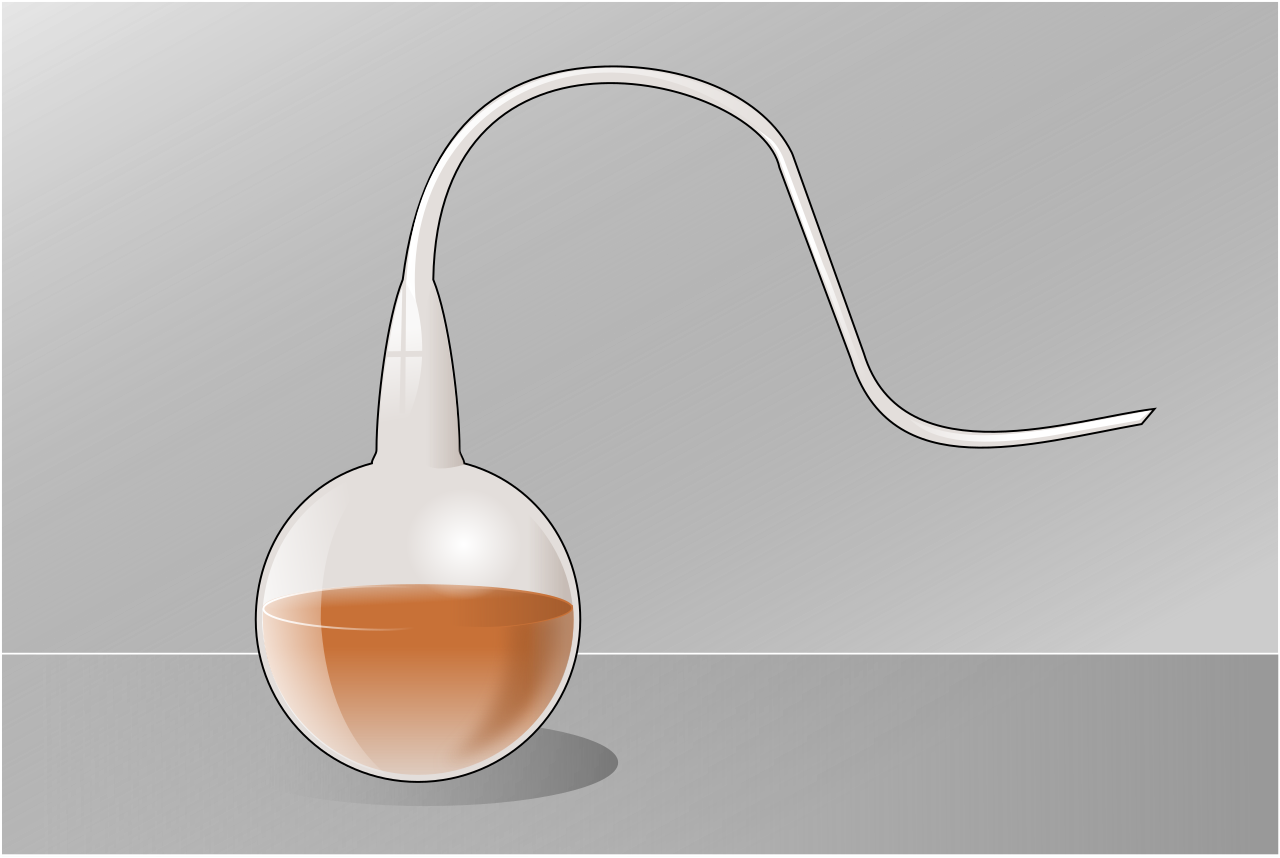
\includegraphics[width=.4\linewidth]{img/1280px-Coldecygne.svg.png}
	\caption{Imagem ilustrativa de um frasco bico-de-cisne, utilizado por Pasteur}
	\caption*{\textit{Fonte:} \href{https://en.wikipedia.org/wiki/Swan_neck_flask}{Wikipédia}}
	\label{bico-de-cisne}
\end{figure}

Para os propósitos deste texto, os termos \textit{abiogênese} e \textit{geração espontânea} serão utilizados intercambiavelmente, muito embora a geração espontânea descreva o pensamento segundo o qual frequentemente, organismos vivos poderiam surgir por meio de um processo reproduzível que faria parte do ciclo de vida de determinadas espécies, enquanto abiogênese descreve um processo pelo qual um único organismo vivo surge espontaneamente. Enquanto a geração espontânea seja hoje em dia uma hipótese completamente descartada, a abiogênese é uma maneira de se referir ao evento que gerou a primeira forma viva da Terra \cite{vlaardingerbroek2010abiogenesis}.

\subsection{Fungos}
Fungos são um reino de organismos eucarióticos, que englobam desde leveduras unicelulares até organismos multicelulares complexos, como cogumelos. No ambiente, atuam principalmente como decompositores de matéria orgânica morta, ainda que suas funções estendam-se muito além, como no processo de \textit{micorriza}, uma associação com raízes de plantas que provê-las um melhor acesso a nutrientes do solo. \cite{buckley2020fungal}. Fungos também estão associados a diversas doenças infecciosas em seres humanos, principalmente relacionadas a contaminação alimentar por mofo em pacientes imunossuprimidos \cite{Benedict2016}.

\subsection{Objetivo}
O objetivo deste experimento foi o estudo do surgimento de fungos e microorganismos em caldos nutritivos associados com diferentes formas de armazenamento e vedação.

\section{Materiais}
Para a realização do experimento foram utilizados os seguintes materiais
\begin{itemize}
	\item 3 placas de Petri
	\item 2 colheres de sopa de amido de milho
	\item 1 saco plástico furado com elástico/prendedor para fechar
	\item 1 béquer
	\item 1 tripé e tela de amianto
	\item 1 baqueta de vidro
	\item 1 bico de Bunsen
	\item 250 mL de água de torneira
\end{itemize}

\section{Procedimento experimental}
O amido de milho foi misturado à água e aquecido com o bico de Bunsen até formar um caldo de consistência levemente viscosa, que então foi distribuído igualmente em quatro recipientes (duas placas de Petri com tampa, e uma com a tampa separada, formando quatro) seguindo a seguintes orientações:
\begin{itemize}
	\item Uma, denominada \textbf{Placa 1}, foi imediatamente tampada após receber o caldo
	\item Outra, denominada \textbf{Placa 2}, foi reservada até resfriar, e então tampada
	\item Outra, denominada \textbf{Placa 3}, foi inserida destampada em um saco plástico fechado com elástico e furado
	\item A última, denominada \textbf{Placa 4}, foi deixada destampada, em completo contato com o ambiente externo
\end{itemize}
As placas foram acompanhadas e fotografadas durante o período de uma semana. Ao final deste, registrou-se microscopicamente uma delas.

\section{Resultados}

\subsection{Estado inicial}
\begin{figure}[H]
	\centering
	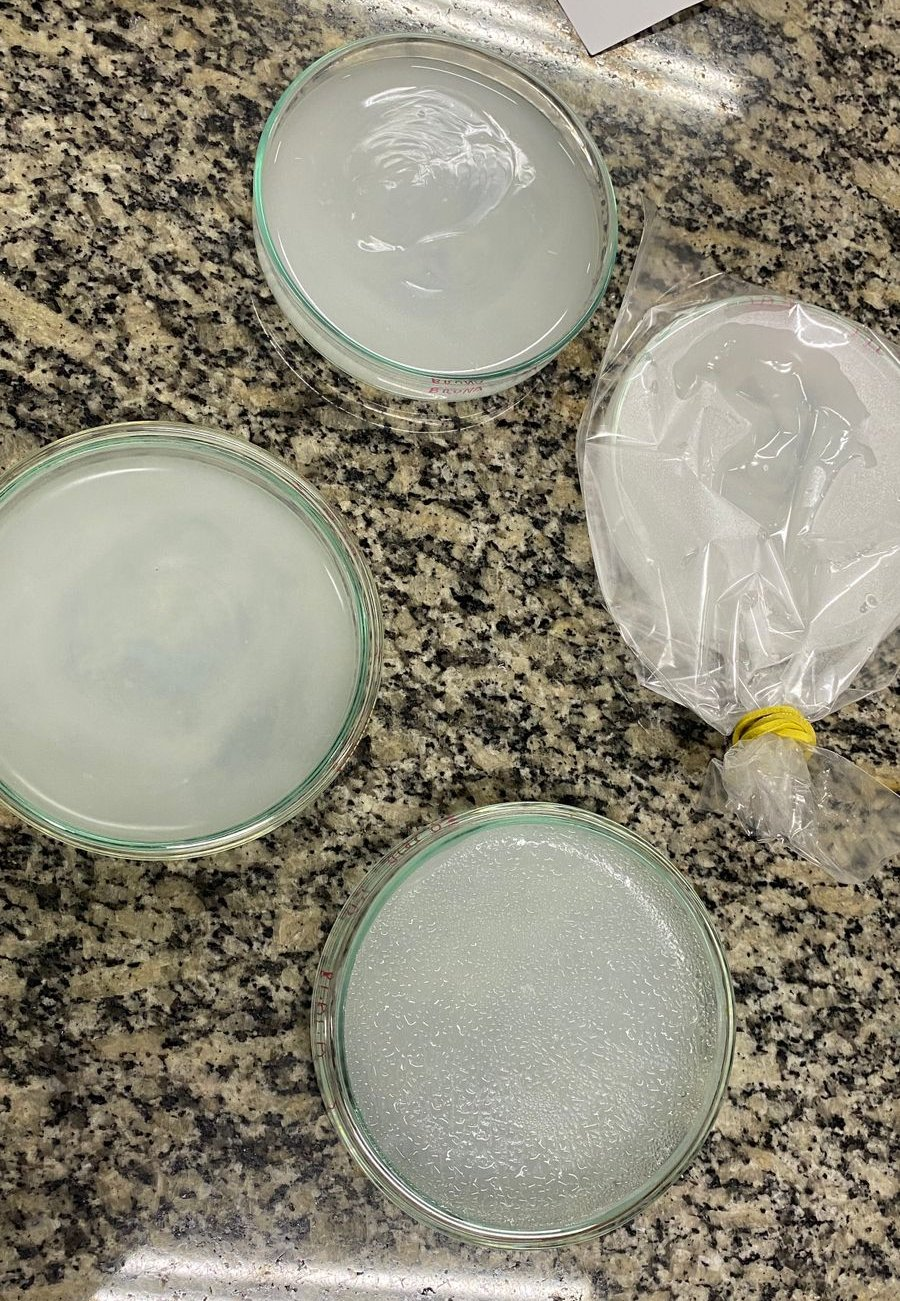
\includegraphics[width=0.5\linewidth]{img/p1234_inicial.jpeg}
	\caption{Observação das placas no início do experimento. Topo: \textbf{Placa 4}, centro-esquerda: \textbf{Placa 2}, centro-direita: \textbf{Placa 3}, em baixo: \textbf{Placa 1}}
	\label{p1234_inicial}
\end{figure}

Todas as placas tinham a mesma coloração, sendo ambientes, no momento, praticamente iguais.

\subsection{Primeira observação, cinco dias após o início}
\begin{figure}[H]
	\centering
	\subcaptionbox{Placa 1}{
		\label{p1_obs1}
		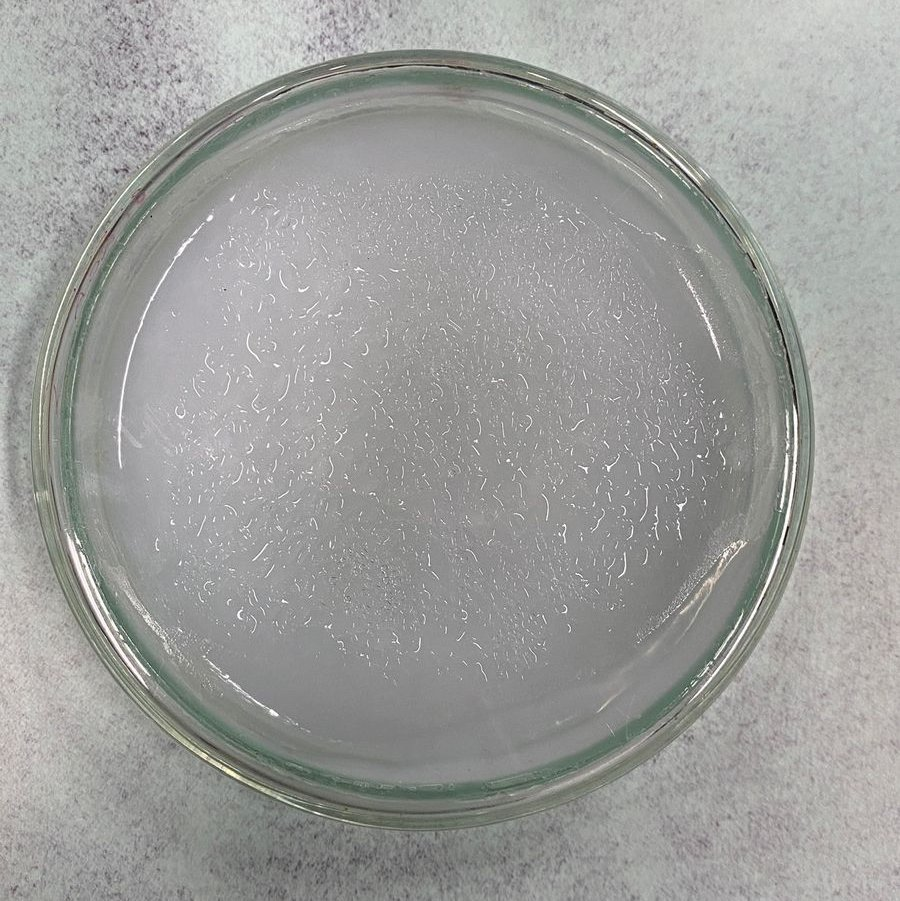
\includegraphics[width=.45\linewidth]{img/p1_obs1.jpeg}\hfill
	}
	\subcaptionbox{Placa 2}{
		\label{p2_obs1}
		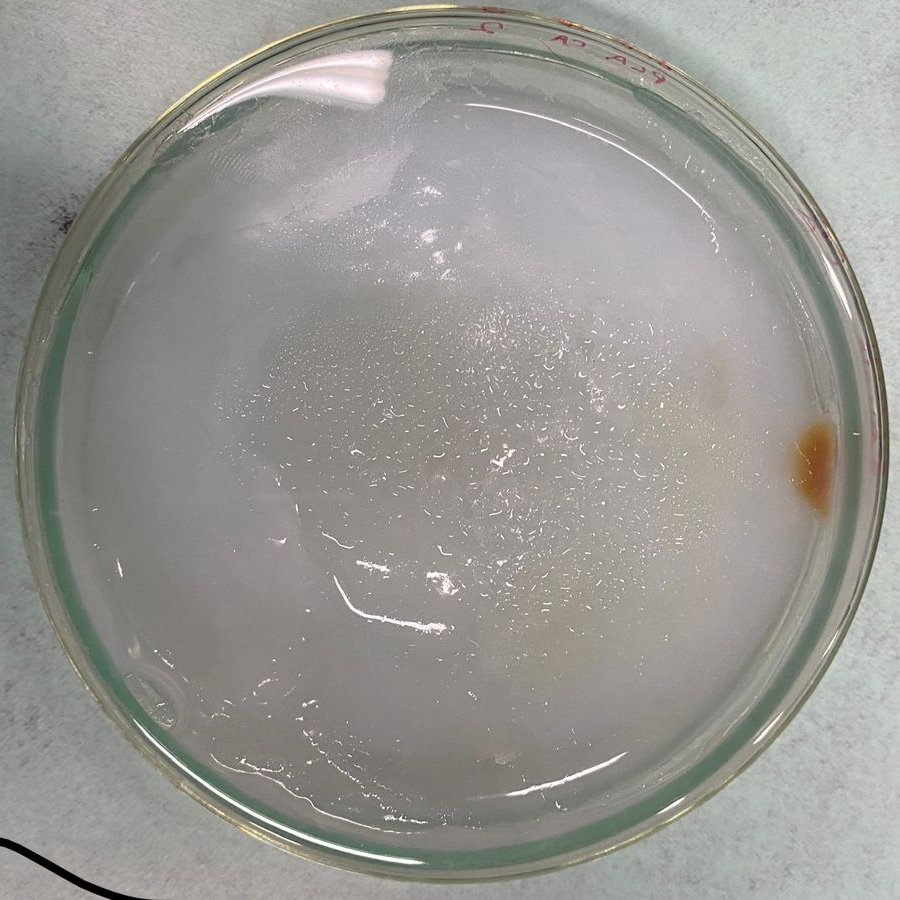
\includegraphics[width=.45\linewidth]{img/p2_obs1.jpeg}\hfill
	}
\end{figure}
\begin{figure}[H]
	\centering
	\ContinuedFloat
	\subcaptionbox{Placa 3}{
		\label{p3_obs1}
		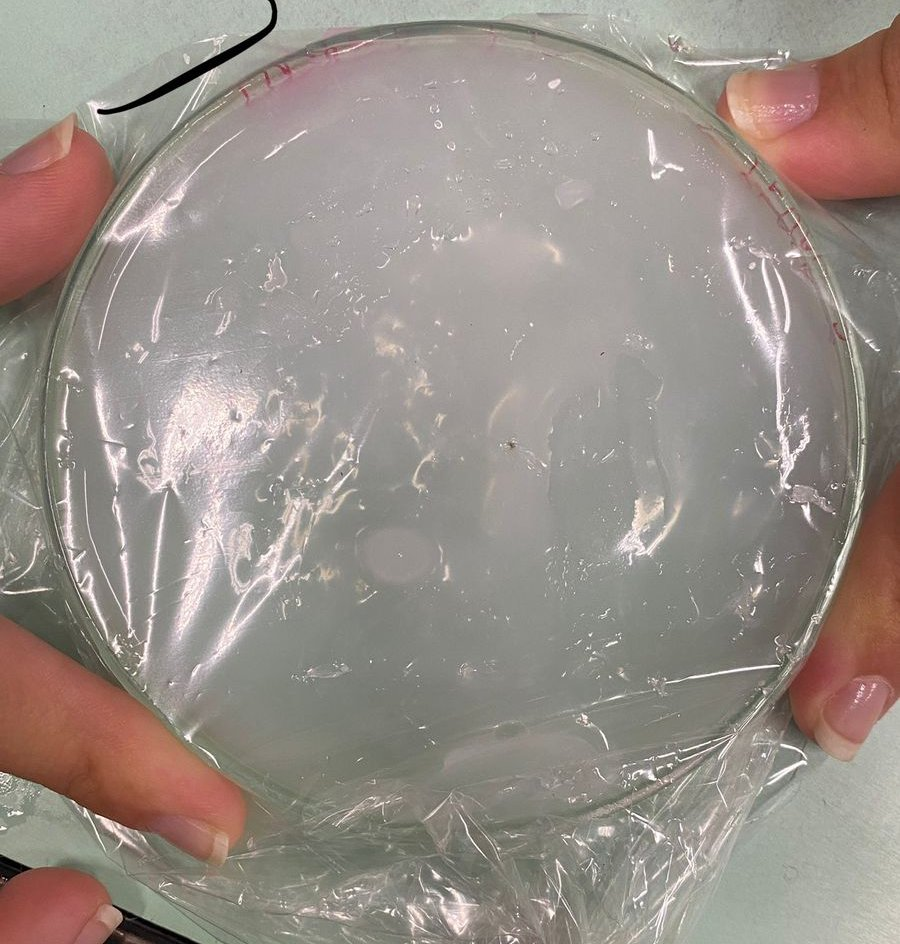
\includegraphics[width=.45\linewidth]{img/p3_obs1.jpeg}\hfill
	}
	\subcaptionbox{Placa 4}{
		\label{p4_obs1}
		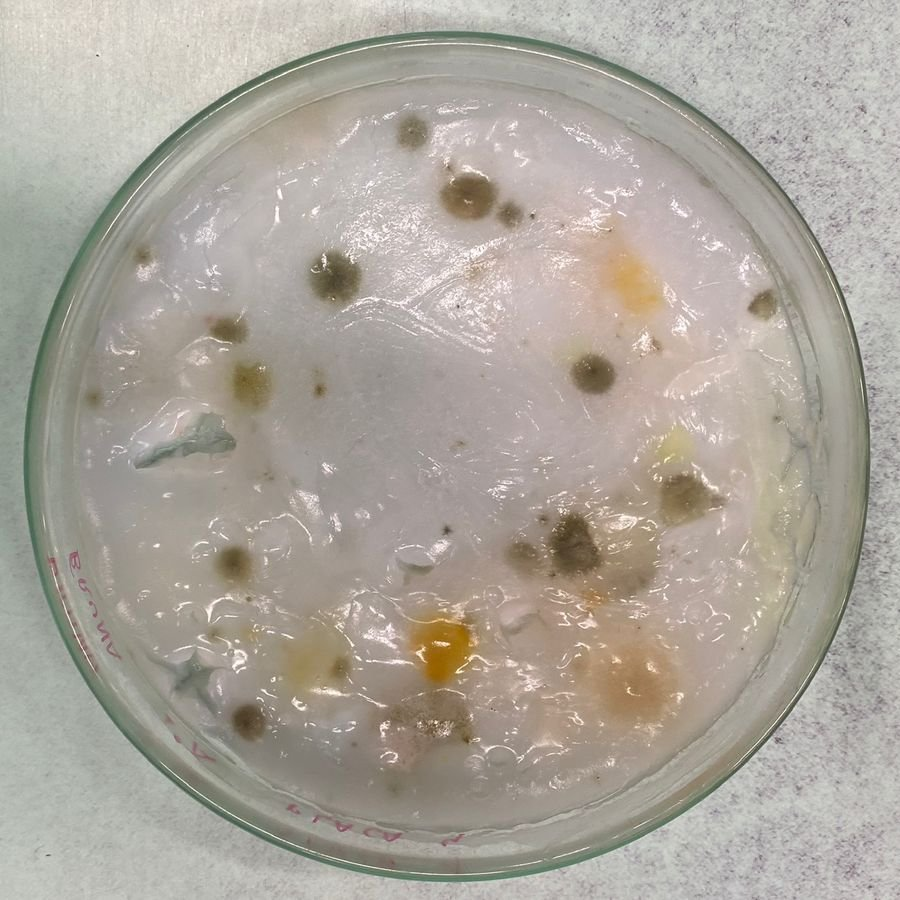
\includegraphics[width=.45\linewidth]{img/p4_obs1.jpeg}\hfill
	}
	\caption{Fotos das placas como estavam cinco dias após o início do experimento. As imagens podem conter artefatos de riscos adicionados virtualmente após sua captura com o intuito de identificação das fotos.}
	\label{obs1}
\end{figure}

Pode-se perceber que houve surgimento substantivo de formas vivas na placa 4 e a aparição de uma mancha na placa 2.
As manchas na placa 3 decorrem de reflexo da caneta utilizada para marcar as placas.

\subsection{Segunda observação, sete dias após o início}
\begin{figure}[H]
	\centering
	\captionsetup[subfigure]{justification=centering}
	\subcaptionbox{Placa 1}{
		\label{p1_obs2}
		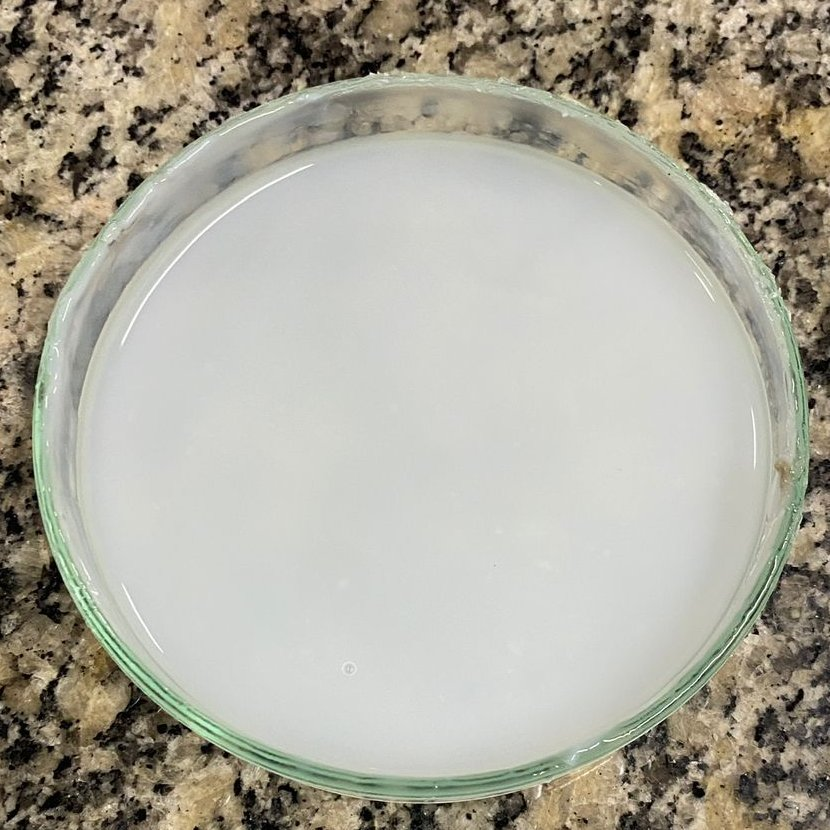
\includegraphics[width=.45\linewidth]{img/p1_obs2.jpeg}\hfill
	}
	\subcaptionbox{Placa 2}{
		\label{p2_obs2}
		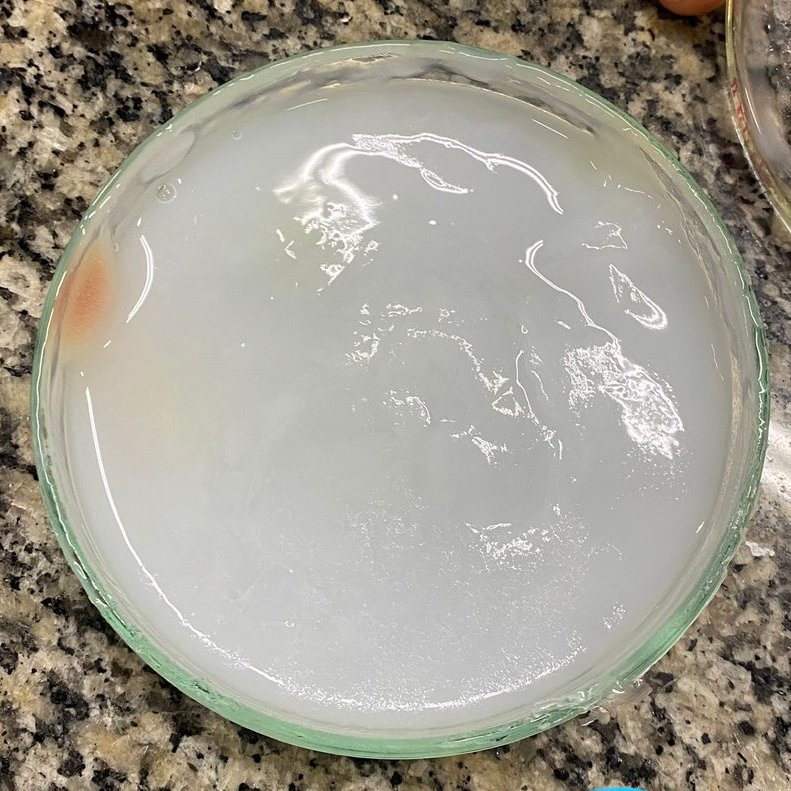
\includegraphics[width=.45\linewidth]{img/p2_obs2.jpeg}\hfill
	}\\
\end{figure}
\begin{figure}[H]
	\captionsetup[subfigure]{justification=centering}
	\centering
	\ContinuedFloat
	\subcaptionbox{Placa 3}{
		\label{p3_obs2}
		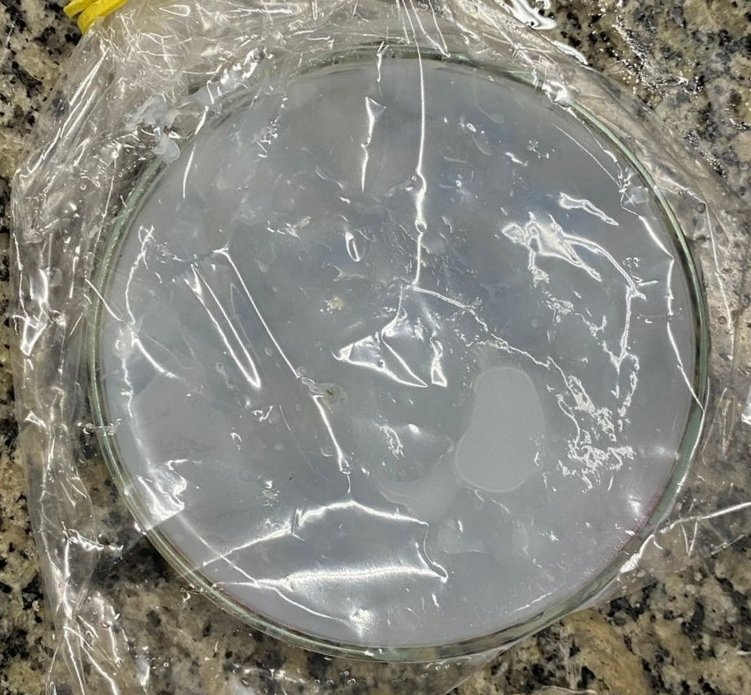
\includegraphics[width=.45\linewidth]{img/p3_obs2.jpeg}\hfill
	}
	\subcaptionbox{Placa 4}{
		\label{p4_obs2}
		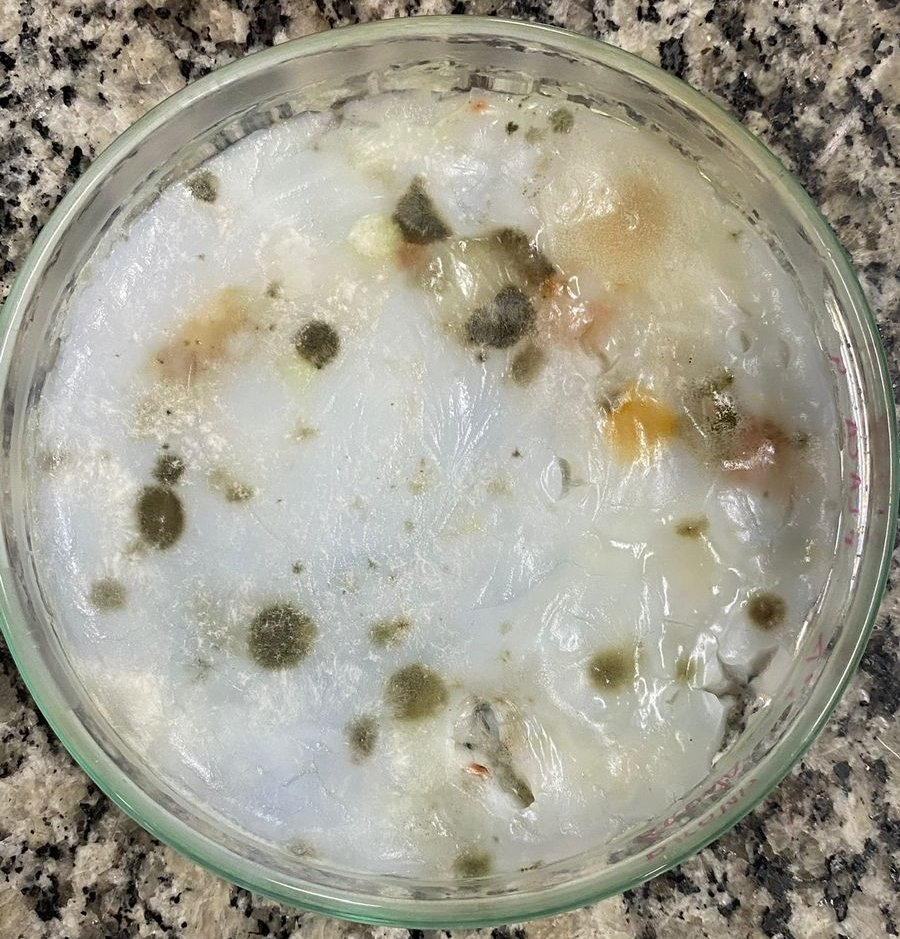
\includegraphics[width=.45\linewidth, max height=.45\linewidth]{img/p4_obs2.jpeg}\hfill
	}

	\caption{Fotos das placas tiradas no sétimo e último dia do experimento.}
\end{figure}

O cenário nas placas continuou parecido com o da figura \ref{obs1}. Nota-se um avanço das formações na placa 1, apenas.

\subsection{Observação microscópica}
\begin{figure}[H]
	\centering
	\captionsetup[subfigure]{justification=centering}
	\subcaptionbox{}{
		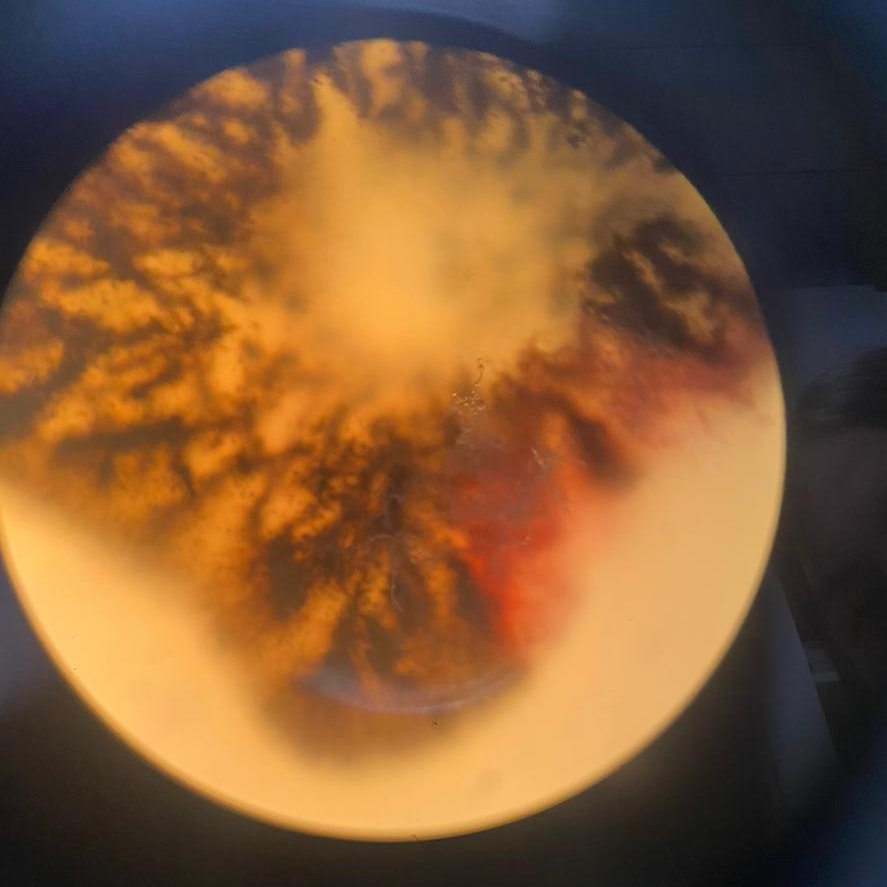
\includegraphics[width=.45\linewidth]{img/mic_1.jpeg}\hfill
	}
	\subcaptionbox{}{
		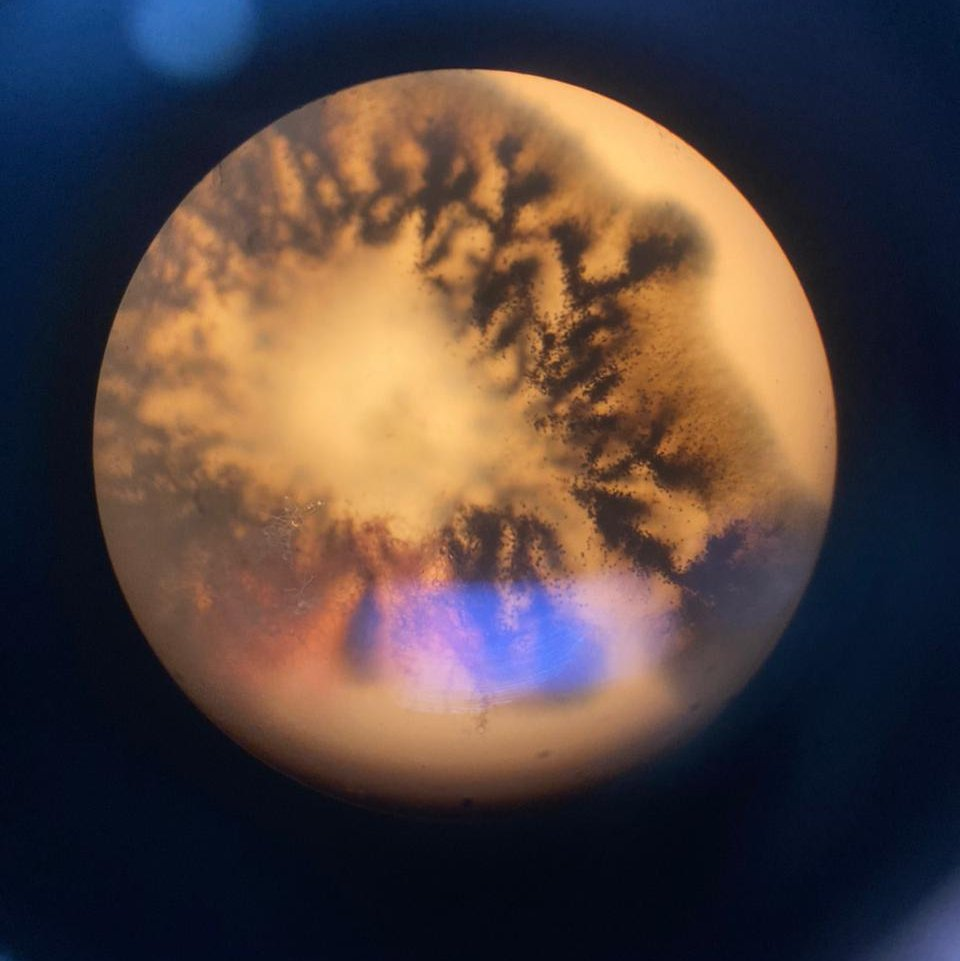
\includegraphics[width=.45\linewidth]{img/mic_2.jpeg}\hfill
	}
	\caption{Fotografias da observação de uma das placas no microscópio}
	\label{mic}
\end{figure}

\section{Discussão}
Pôde-se perceber que, quanto maior a exposição do ambiente interno ao ambiente externo em temperatura ambiente, maior foi o crescimento de microorganismos. A placa 1, que teve sua exposição externa minimizada, não observou crescimento visível de vida. A placa 2, que teve alguma exposição ao ambiente antes de ser tampada, observou pequeno crescimento de vida, centrado em uma só mancha nos cantos da placa, proveniente do período onde teve contato externo com uma temperatura interna tolerável para tais microorganismos. Por fim, a placa 4, que teve máxima exposição externa, teve um crescimento muito maior que todas as outras, com diversas manchas que cobriam toda a superfície.

No caso da placa 3, houve um erro no procedimento, visto que o intento era que a circulação de ar através dos furos fizesse com que microorganismos surgissem no caldo nutritivo. Evidente pela abstenção de formas vivas visíveis nela, isso não ocorreu, provavelmente devido a uma baixa quantidade de furos ou pelos furos terem sido feitos cedo demais e remendados pelo calor.

Provavelmente, se o recorte temporal do experimento fosse maior, microorganismos poderiam ter surgido em todas as placas. A vedação das placas fechadas não era perfeita, e com o passar do tempo eventuais colônias presentes teriam aumentado de tamanho e tornado-se mais perceptíveis. Além disso, a isenção de vida visível em algumas placas não implica que não haja vida nelas - mas sim, que não havia vida que se manifestasse de maneira a ser visível a olho nu.

Outro problema que pode ter acontecido no experimento é a contaminação das placas de Petri, que teriam induzido o crescimento de uma forma viva que não estaria lá caso a placa tivesse sido completamente esterilizadas.

Os resultados conformam-se com proposições amplamente aceitas da biologia: de que microorganismos provém de um contato com o ar e um ambiente externo onde já viviam. Essa proposição já foi provada em 1859, com o experimento do bico-de-cisne de Pasteur (veja \S\ref{intro-surg-vida}), e continua sendo a forma mais aceita para explicar a aparição de seres vivos dentro da ciência moderna. Também conformam-se com o consenso científico de que a maioria dos microorganismos que potencialmente poderiam contaminar o meio 2 foram mortos por sua alta temperatura, implicando que teriam uma faixa de temperatura necessária para sobreviver: entre o "muito quente", como na placa 2, e o "muito frio", como em \textit{freezers} e geladeiras, já que a velocidade de todas as reações químicas diminui conforme a temperatura do ambiente diminui, incluindo as reações biológicas de decomposição.

Essas conclusões também reiteram a recomendação comum do uso de embalagens hermeticamente fechadas para o armazenamento de alimentos - com o intuito de diminuir o contato com um ambiente externo potencialmente contaminado - e do aquecimento de alimentos potencialmente contaminados, como ovos com salmonela, ambas a fim de reduzir o número de infecções resultantes de microorganismos danosos à saúde humana. A higiene, não só dos alimentos em si, mas também de toda a cadeia de transporte, venda e consumo, é um tópico de grande discussão, visto que muitas vezes ela é insuficiente para garantir a integridade e esterilidade deles \cite{coelho_milagres_martins_azeredo_santana_2010, balbani2001contaminaccao}.

A observação microscópica revelou uma miríade de pequenos organismos filamentosos - provavelmente fungos \cite{buckley2020fungal}, ainda que fosse necessária uma análise microbiótica mais detalhada para que houvesse mais certeza nessa afirmação, mas que está além do escopo deste experimento. Como já dito, fungos estão relacionados a infecções potencialmente mortais em seres humanos \cite{Benedict2016}, de difícil identificação e tratamento, reforçando essa mensagem da importância da higiene.

\section{Conclusão}
Apesar não ter sido um estudo preciso em relação ao isolamento externo de suas amostras, esse experimento mostrou-se, na maior parte, conivente com teorias aceitas da biologia de que microorganismos provém de contato com o ar, e logo, quanto mais exposição externa tiver um meio, maior será o número de microorganismos que surgirão nele proporcionais a fatores externos como temperatura.

\printbibliography

\end{document}

